\section{Empirical Evidence}



\begin{frame}[label=actual_distribution]{Source of Incentive}
    \framesubtitle{\textcolor{structure}{Actual distritution is similar to (Imperfect Risk Adjustment) example.}}
    \begin{figure}
        \includegraphics[width=0.6\textwidth]{figures/images/capitation_spending_distribution_togather.png}
    \end{figure}
    \hyperlink{example_distribution}{\beamergotobutton{Example Distribution}}
\end{frame}

\begin{frame}[label=source_of_incentive]{Source of Incentive}
    \framesubtitle{\textcolor{structure}{Actual distritution is similar to (Imperfect Risk Adjustment) example.}}
    Why is the capitation so concentrated?
    \begin{itemize}
        \item A byproduct of the \textit{conventional} risk adjustment.
        \item It runs a regression on TM spendings over the condition dummaies.
        \item $R^2$ is 0.1\footnote{On the individual level, accroding to \textit{Report to Congress: Risk Adjustment in MA, 2021, MedPAC}}, 90\% of the variation is not explained by the model.
        \item \hyperlink{example_start}{This example} illustrates how centratation happens.
    \end{itemize}
\end{frame}


\begin{frame}{Plan Design and Outside Option}
    \label{version1}
    \framesubtitle{\textcolor{structure}{A generous outside option is always available: TM-Medigap}}
    \begin{table}[ht]
    \centering
    \caption{Comparison of Popular MA and Medigap plans in Suffolk County 2016}
    \begin{tabular}{|l|c|c|c|}
    \hline
    \multicolumn{4}{|c|}{\textbf{Medicare Advantage}} \\
    \hline
    Plan Code & Premium & Out-Of-Pocket & Additional Benefits \\
    \hline
    H3370-032 & \$372  & \multirow{3}{*}{\parbox{4cm}{Copay \& Coinsurance \footnote{Amounts paid by the insured, which increase with the medical services rendered.} \\ with minor variations}} & Dental, Vision, Hearing   \\
    \cline{1-2}\cline{4-4}
    R5342-001 & \$0 & & Vision, Hearing           \\
    \cline{1-2}\cline{4-4}
    H4922-001 & \$0 & & Dental, Vision           \\
    \multicolumn{4}{|c|}{\ldots} \\
    \hline
    \multicolumn{4}{|c|}{\textbf{TM-Medigap}} \\
    \hline
    Plan Code & Premium & Out-Of-Pocket & Additional Benefits \\
    \hline
    Plan C & \$3108  & No \footnote{Charges may apply for special situations like Foreign Travel, but are omitted for brevity.} & No \\
    \hline
    \end{tabular}
\end{table}
    
    
    
    \hyperlink{version2}{\beamergotobutton{another version}}
\end{frame}

\begin{frame}{Plan Design and Outside Option}
    \framesubtitle{\textcolor{structure}{A generous outside option is always available: TM-Medigap}}
    \begin{itemize}
        \item \textbf{TM-Medigap:} \textit{high} generosity; \textit{high} premium.
        \item \textbf{MA:} \textit{low} generosity; \textit{low} premium.
        \vfill
        \item \textbf{TM-Medigap:} degined by CMS, consistently offered in all markets.
        \item \textbf{MA:} designed by MA firms.
    \end{itemize}
    \vfill
\end{frame}


\begin{frame}{MCBS Data}

    \begin{itemize}
        \item \textit{Medicare Current Beneficiary Survey}, an annual survey.
        \item Capturing individual level health and financial details.
    \end{itemize}
    \vfill
   Will leverage this data to substantiate conditions on consumers' hetrogeneity.
    \begin{itemize}
        \item \textcolor{structure}{Consumers' health perceptions provide extra insight into spending.}
        \item \textcolor{structure}{Health perceptions influence individual preferences for generosity.}
    \end{itemize}

\end{frame}



\begin{frame}{MCBS Interview}
\begin{figure}
    \centering
    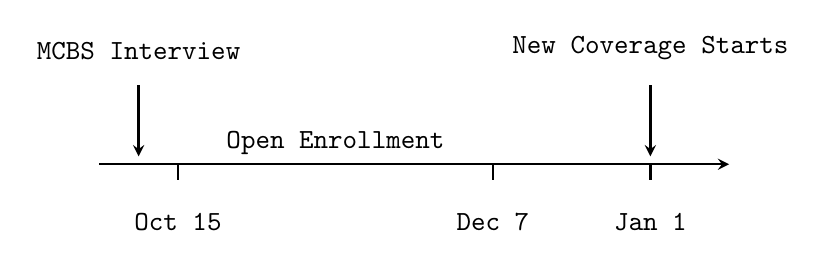
\begin{tikzpicture}
    % Draw horizontal line
    \draw[->, >=stealth, thick] (0,0) -- (8,0);
    
    % Draw vertical lines for the dates
    \draw[thick] (1,-0.2) -- (1,0);
    \draw[thick] (5,-0.2) -- (5,0);
    \draw[thick] (7,-0.2) -- (7,0);
    
    % Place the date labels
    \node[align=center, below] at (1,-0.5) {Oct 15};
    \node[align=center, below] at (5,-0.5) {Dec 7};
    \node[align=center, below] at (7,-0.5) {Jan 1};

    % Add "Open Enrollment" label above the line between Oct 15 and Dec 7
    \node[align=center, above] at (3,0) {Open Enrollment};

    % Add arrow and label for "MCBS Interview" to the left of Oct 15
    \draw[->, >=stealth, thick] (0.5,1) -- (0.5,0.1);
    \node[align=center, above] at (0.5,1.2) {MCBS Interview};

    % Add arrow and label for "New Coverage Starts" at Jan 1
    \draw[->, >=stealth, thick] (7,1) -- (7,0.1);
    \node[align=center, above] at (7,1.2) {New Coverage Starts};
\end{tikzpicture}
    \caption{Annual Timeline}
\end{figure}
\end{frame}


\begin{frame}{MCBS Interview}

    Interview Question: \texttt{`General health compared others same age.'}

    Response Options:
    \begin{figure}
        \centering
        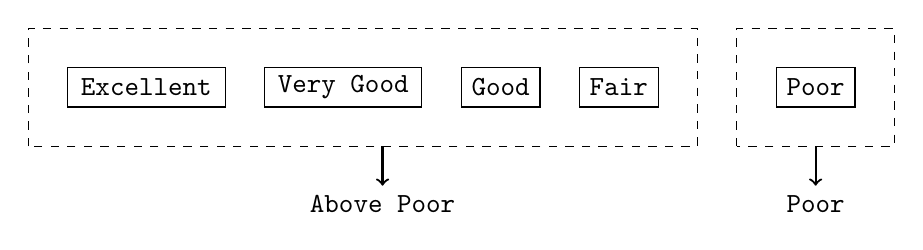
\begin{tikzpicture}
    % Define the font style
    \tikzstyle{every node}=[font=\ttfamily]
  
    % Draw the rectangles for each answer option
    \draw (0,0) rectangle (2,0.5) node[midway] {Excellent};
    \draw (2.5,0) rectangle (4.5,0.5) node[midway] {Very Good};
    \draw (5,0) rectangle (6,0.5) node[midway] {Good};
    \draw (6.5,0) rectangle (7.5,0.5) node[midway] {Fair};
    \draw (9,0) rectangle (10,0.5) node[midway] {Poor};
  
    \pause
    % Draw the dashed rectangles around the grouped answer options
    \draw[dashed] (-0.5,-0.5) rectangle (8,1);
    \draw[dashed] (8.5,-0.5) rectangle (10.5,1);
  
    % Add arrows pointing downwards from the middle of the dashed rectangles
    \draw[->, thick] (4,-0.5) -- (4,-1) node[below] {Above Poor};
    \draw[->, thick] (9.5,-0.5) -- (9.5,-1) node[below] {Poor};
\end{tikzpicture}
    \end{figure}

    \onslide<2->{
        Will use following variables from MCBS:

        \begin{itemize}
            \item \textbf{Health Perception Response}
            \item \textbf{Next Year Spending}
            \item \textbf{Next Year MA Enrollment}
        \end{itemize}
    }

\end{frame}

\begin{frame}{Next Year Spending}
    \framesubtitle{\textcolor{structure}{Consumers' health perceptions provide extra insight into spending.}}
    \begin{figure}
        \centering
        \includegraphics[width=1\textwidth]{figures/images/next_year_spending_distribution_grouped.png}
    \end{figure}
\end{frame}

\begin{frame}{Next Year Spending}
    \framesubtitle{\textcolor{structure}{Consumers' health perceptions provide extra insight into spending.}}
    Consumers have some private information.
    \vfill

    \textbf{Poor Group:}
    \begin{itemize}
        \item Has notably higher spendings, \textit{irrespective of} plan choices.
        \item Poses a risk for MA losses, under the current Risk Adjustment.
    \end{itemize}

\end{frame}

\begin{frame}{Next Year MA Enrollment}
    \framesubtitle{\textcolor{structure}{Health perceptions influence individual preferences for generosity.}}
    \begin{itemize}
        \item MA plans have lower generosities than TM-Medigap.
    \end{itemize}
    \vfill
    \centering
    \begin{tabular}{p{4cm}|p{2cm}} 
        \textbf{Response Group} \newline \textbf{on General Health} & \textbf{MA Ratio} \newline \textbf{Next Year} \\
        \hline
        Poor & 0.216 \\
        Above Poor & 0.283 \\
        \hline \hline
        \textit{Overall} & 0.279 \\
    \end{tabular}
\end{frame}


\begin{frame}{Regression Analysis}
    \framesubtitle{\textcolor{structure}{Health perceptions influence individual preferences for generosity.}}
    \begin{table}[!htbp] \centering 
        \caption{Logistic Regression Results} 
      \begin{tabular}{@{\extracolsep{5pt}}lD{.}{.}{-3}D{.}{.}{-3} } 
      \\[-1.8ex]\hline 
      \hline \\[-1.8ex] 
       & \multicolumn{2}{c}{\textit{MA\_next\_year}} \\ 
      \cline{2-3} 
      \\[-1.8ex] & \multicolumn{1}{c}{Coefficient} & \multicolumn{1}{c}{Std. Error} \\ 
      \hline \\[-1.8ex] 
      \textbf{GENHELTH\_poor} & -0.601^{***} & (0.167) \\ 
       log\_income & -0.373^{***} & (0.031) \\ 
       race\_white & -0.401^{***} & (0.069) \\ 
       female & -0.033 & (0.046) \\ 
       age & -0.012^{***} & (0.003) \\ 
       edu\_high & -0.367^{***} & (0.049) \\ 
      \hline \\[-1.8ex] 
      \textit{Note:}  & \multicolumn{2}{r}{$^{*}$p$<$0.1; $^{**}$p$<$0.05; $^{***}$p$<$0.01} \\ 
      \end{tabular} 
    \end{table} 
    
\end{frame}

\begin{frame}{Results Summary}
    \framesubtitle{\textcolor{structure}{Health perceptions influence individual preferences for generosity.}}
    \textbf{Regression:}
        \begin{itemize}
            \item Various factors influence consumer's MA enrollment choice.
            \item Health perception stands out as a significant predictor.
        \end{itemize}
        \vfill
        \pause
        \textbf{Implication:}
        \begin{itemize}
            \item Under current plan designs, the healthy tend to self-select into MA.
            \item Under current Risk Adjustment, they tend to be very profitable.
        \end{itemize}
\end{frame}

\begin{frame}{Sum Up}
    \textbf{Demand Side:}
    \begin{itemize}
        \item Consumers' feeling about their health can:
        \begin{itemize}
            \item provide information about spending
            \item influence their plan choice
        \end{itemize}
    \end{itemize}
    \vfill
    \pause
    \textbf{Supply Side:}
    \begin{itemize}
        \item A generous outside option (TM-Medigap) is always available.
        \item MA firms design \textit{cheap} low generosity plans to attract profitable consumers.
        \item Incentive originates from the current Risk Adjustment.
    \end{itemize}
    \pause
    \vfill
    \textbf{CMS:}
    \begin{itemize}
        \item Risk Adjustment to elminate selection, but it was \textit{not} very successful.
        \item Overpaid consumers are more likely to join MA, under firms' strategy.
        \item Consequently, CMS overpays MA firms.
    \end{itemize}
\end{frame}


\begin{frame}[label=explain_overpayment]{Explaining the Overpayment}
    \textbf{Overpayment:}
    \begin{itemize}
        \item Difference between Average Spending and Average Capitation.
        \item MA: Average Spending: \$6012. Average Capitation: \$8847.
        \item Nearly 30\% overpaid – an unreasonably high margin.
    \end{itemize}
    \hyperlink{overpayment_distribution}{\beamergotobutton{Distribution}}
    \hyperlink{tab:personal_level_summary}{\beamergotobutton{Stats Table}}
    \vfill
    \textbf{Our story:}
    \begin{itemize}
        \item Explains overpayment, \textit{at least partially}, is caused by selection.
        \item Selection targets the healthy, regardless of their capitation.
        \item This makes strategy simple and feasible.
        \item Root cause: current Risk Adjustment.
    \end{itemize}
\end{frame}


